\chapter{Matemáticas Básicas}
\lipsum[11-20]
\section*{\hypertarget{Id1}{\hyperlink{Id11}{Álgebra básica}}}
\addcontentsline{toc}{section}{Álgebra básica}
\markright{Álgebra básica}
\begin{Def}
Una expresión algebrica es un objeto matemático formado por operaciones matemáticas entre diferentes variables y números.\footnote[5]{Esta definición no es convencional.}  
\end{Def}
Considere un ejemplo de una expresión algebraica\index{algebraica} compleja\footnote{Este ejemplo fue tomado del álgebra de Baldor.}
\begin{displaymath}
\sqrt{\frac{ab}{c}}+2(b-a)\sqrt{\frac{9b}{a^2}}-3(c-b)\sqrt[3]{\frac{b}{c}}
\end{displaymath}
Ahora vamos a evaluar la expresión anterior en $a=4$, $b=9$ y $c=25$:
\begin{displaymath}
\sqrt{\frac{ab}{c}}+2(b-a)\sqrt{\frac{9b}{a^2}}-3(c-b)\sqrt[3]{\frac{b}{c}}
=
\sqrt{\frac{4\cdot 9}{25}}+2(9-4)\sqrt{\frac{9\cdot 9}{4^2}}-3(25-9)\sqrt[3]{\frac{9}{25}}
\end{displaymath}
\begin{displaymath}
=
\sqrt{\frac{4\cdot 9}{25}}+2(9-4)\sqrt{\frac{9\cdot 9}{4^2}}-3(25-9)\sqrt[3]{\frac{9}{25}}
\end{displaymath}
\begin{align*}
\sqrt{\frac{ab}{c}}+2(b-a)\sqrt{\frac{9b}{a^2}}-3(c-b)\sqrt[3]{\frac{b}{c}}= & \sqrt{\frac{4\cdot 9}{25}}+2(9-4)\sqrt{\frac{9\cdot 9}{4^2}}-3(25-9)\sqrt[3]{\frac{9}{25}}\\
=& \sqrt{\frac{4\cdot 9}{25}}+2(9-4)\sqrt{\frac{9\cdot 9}{4^2}}-3(25-9)\sqrt[3]{\frac{9}{25}}
\end{align*}
Un ejempplo de una ecuación importante que involucra expresiones algebraicas es la referente al teorema de pitagoras:
\begin{equation}\label{EcuacionPitagoras}
c^2=a^2+b^2.
\end{equation}
Dado que la ecuación \eqref{EcuacionPitagoras} se cumple entonces en un triángulo con catetos 4 y 3 su hipotenusa es 5.\\
Un polinomio lineal se define como $p(x)=ax+\dfrac{c}{d}$ donde $a$  y $b$ son números reales. En general:
\begin{Def}[Definición de Polinomio]
Un polinomio es una expresión algebrica de la forma:
$$p(x)=a_nx^n+ a_{n-1}x^{n-1}+\cdots+a_1x+a_0,$$
donde $a_n\neq 0$.
\end{Def}
\begin{Prop}[Teorema del residuo]
El residuo de dividir $P(x)$ por $x-c$ es igual a $P(c)$.
\end{Prop}
Ahora veremos como construir la siguiente imagen usando tablas:
\begin{figure}[H]
\centering
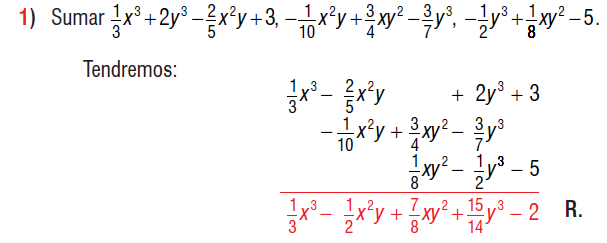
\includegraphics[scale=1.2]{Imagen1}
\caption{Fragmento tomado del Álgebra de Baldor}
\end{figure}
\begin{displaymath}
\renewcommand{\arraystretch }{2}
\begin{array}{ccccc>{\columncolor{gray}}p{1cm}}
\dfrac{1}{3}x^3&-\dfrac{2}{5}x^2y&&+2y^3&+3&\\
&\cellcolor{gray}\textcolor{white}{-\dfrac{1}{10}x^2y}&+\dfrac{3}{4}xy^2&-\dfrac{3}{7}y^3&&\\
&&\dfrac{1}{8}xy^2&-\dfrac{1}{2}y^3&-5&\\ \cline{1-5}
&&&&& \textcolor{white}{\textbf{R.}}
\end{array}
\end{displaymath}
% Please add the following required packages to your document preamble:
% \usepackage[table,xcdraw]{xcolor}
% Beamer presentation requires \usepackage{colortbl} instead of \usepackage[table,xcdraw]{xcolor}
\lipsum[1-10]
\section*{Vectores y Matrices}
\addcontentsline{toc}{section}{Vectore y Matrices} % Añade al índice
\markright{Vectores y Matrices}
\begin{figure}[H]
\centering 
\includegraphics[scale=0.5]{Simetria}
\caption{Esta imagen fue tomada de la página de internet \href{https://www.freepik.com/}{$\underline{Enlace}$}}
\end{figure}
\begin{center}
\fbox{
\begin{minipage}{0.7\textwidth}
Aunque no lo parezca, una imagen\index{imagen} no es más que una tabla de números para un computador.
\end{minipage}
}
\end{center}
\begin{Def}[Vector]
Se define un vector $x$ de $n$ elementos como una lista de $n$ números dispuestos de la siguiente forma:
\begin{displaymath}
x=
\begin{pmatrix}
x_1\\
x_2\\
\vdots\\
x_n
\end{pmatrix}
\end{displaymath}
Se denota que $x\in\mathbb{R}^n$.
\end{Def}
\begin{table}
\centering
\begin{tabular}{|c|c|c|}
\hline
1 & 2 & 3\\
\hline
\end{tabular}
\end{table}